\documentclass{beamer}
% Required packages
\usepackage{amsmath}
\usepackage{physics}
\usepackage{graphicx}
\usepackage{siunitx}
\usepackage{xcolor}
% Set image search paths
\graphicspath{{../images/}{../../shared/images/}}

% Define custom colors for DS9 theme
\definecolor{ds9blue}{RGB}{25,25,112}
\definecolor{ds9gold}{RGB}{218,165,32}
\definecolor{ds9grey}{RGB}{105,105,105}
\definecolor{ds9red}{RGB}{178,34,34}
% Set up the Madrid theme with custom colors
\usetheme{Madrid}
\usecolortheme{whale}
\setbeamercolor{palette primary}{bg=ds9blue,fg=white}
\setbeamercolor{palette secondary}{bg=ds9grey,fg=white}
\setbeamercolor{palette tertiary}{bg=ds9gold,fg=black}
\setbeamercolor{palette quaternary}{bg=ds9red,fg=white}
\setbeamercolor{structure}{fg=ds9blue}
\setbeamercolor{title}{fg=ds9gold}
\setbeamercolor{subtitle}{fg=ds9gold}
\setbeamercolor{frametitle}{bg=ds9blue,fg=white}
\setbeamercolor{block title}{bg=ds9blue,fg=white}
\setbeamercolor{block body}{bg=ds9grey!20,fg=black}

% Title page configuration
\title[Electric Forces \& Fields]{PHYS11 CH18: Electrostatics}
\subtitle{Charges, Fields, Potential, and Capacitors}
\author[Mr. Gullo]{Mr. Gullo}
\date[May 2025]{May, 2025}

% Define sections for outline
\AtBeginSection[]
{
  \begin{frame}
    \frametitle{Outline}
    \tableofcontents[currentsection]
  \end{frame}
}

\begin{document}

% Title page
\begin{frame}
    \titlepage
\end{frame}

% Outline
\begin{frame}
    \frametitle{Presentation Outline}
    \tableofcontents
\end{frame}

\section{Introduction}

% Learning Objectives
\begin{frame}
    \frametitle{Learning Objectives}
    By the end of this presentation, you will be able to:
    \begin{itemize}
        \item Describe the nature of electric charge and its conservation
        \item Apply Coulomb's law to calculate forces between charges
        \item Define and calculate electric fields around charge distributions
        \item Understand electric potential and potential energy concepts
        \item Explain how capacitors work and calculate their capacitance
        \item Solve problems involving electric forces, fields, potential, and capacitors
    \end{itemize}
\end{frame}

\section{Electrical Charges}

% Electrical Charges
\begin{frame}
    \frametitle{Electrical Charges}
    \begin{block}{Key Concepts}
        \begin{itemize}
                    \item Two varieties: \textbf{positive} and \textbf{negative}
            \item Like charges \textbf{repel}, opposite charges \textbf{attract}
        \end{itemize}
    \end{block}
    
    
        \begin{figure}
            \centering
            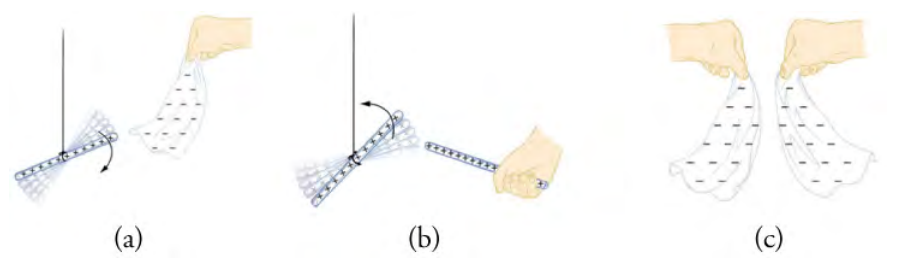
\includegraphics[width=1\linewidth]{phys11-electrostatics-charge-attraction-repulsion.png}
        \end{figure}
    
    
    \begin{block}{Conductors vs. Insulators}
        \begin{itemize}
            \item \textbf{Conductors}: Charges move easily \textbf{Insulators}: Charges cannot move easily
        \end{itemize}
    \end{block}
\end{frame}

% Charge Transfer Methods
\begin{frame}
    \frametitle{Transfer of Charge}
    Three ways to charge objects:
    \begin{enumerate}
        \item \textbf{Charging by contact}
            \begin{itemize}
                \item Direct physical contact between objects
                \item Charges transfer from one object to another
            \end{itemize}
        \item \textbf{Charging by conduction}
            \begin{itemize}
                \item Charges flow through conducting path
            \end{itemize}
        \item \textbf{Charging by induction}
            \begin{itemize}
                \item No contact required
                \item Charge separation due to electric field
            \end{itemize}
    \end{enumerate}
    
    
       \begin{figure}
           \centering
           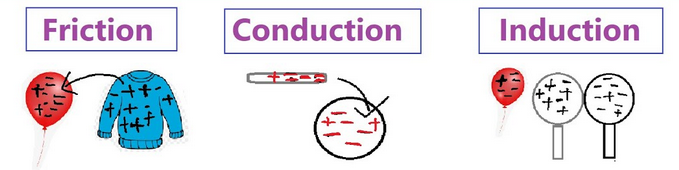
\includegraphics[width=1\linewidth]{phys11-electrostatics-charging-methods.png}
       \end{figure}
    
\end{frame}

% Polarization
\begin{frame}
    \frametitle{Polarization}
    \begin{block}{Polarized Objects}
        \begin{itemize}
            \item A polarized object may be electrically neutral overall
            \item But its charge is \textbf{unbalanced}:
                \begin{itemize}
                    \item One side has excess \textbf{negative} charge
                    \item The other side has equal magnitude of excess \textbf{positive} charge
                \end{itemize}
        \end{itemize}
    \end{block}
    
    
        \begin{figure}
            \centering
            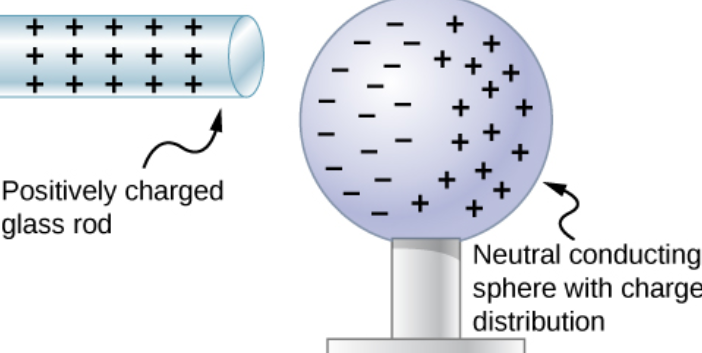
\includegraphics[width=0.75\linewidth]{phys11-electrostatics-polarization.png}
        \end{figure}
    
\end{frame}

\section{Coulomb's Law}

% Coulomb's Law
\begin{frame}
    \frametitle{Coulomb's Law}
    \begin{block}{Definition}
        Coulomb's law describes the electrostatic force between charged particles:
        \begin{equation}
            \vec{F} = \frac{kq_1q_2}{r^2}\hat{r}
        \end{equation}
        where:
        \begin{itemize}
            \item $k = 9 \times 10^9 \, \text{N} \cdot \text{m}^2/\text{C}^2$ (Coulomb constant)
            \item $q_1, q_2$ are the charges
            \item $r$ is the distance between charges
            \item $\hat{r}$ is the unit vector pointing from $q_1$ to $q_2$
        \end{itemize}
    \end{block}
\end{frame}

% Coulomb's Law Properties
\begin{frame}
    \frametitle{Properties of Coulomb's Law}
    \begin{itemize}
        \item \textbf{Inverse square law}: Force $\propto \frac{1}{r^2}$
        \item Force is \textbf{proportional} to the product of charges
        \item Force interpretation:
            \begin{itemize}
                \item $F < 0$ → \textbf{attractive} force
                \item $F > 0$ → \textbf{repulsive} force
            \end{itemize}
        \item Vector nature: Forces act along the line joining the charges
    \end{itemize}
    
    
       \begin{figure}
           \centering
           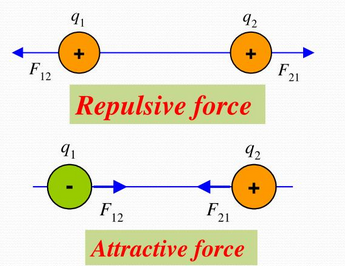
\includegraphics[width=1\linewidth]{phys11-electrostatics-coulomb-force-types.png}
       \end{figure}
    
\end{frame}

\section{Electric Field}

% Electric Field Concept
\begin{frame}
    \frametitle{Electric Field Concept}
    \begin{block}{Definition}
        The electric field defines the force per unit charge in the space around a charge distribution:
        \begin{equation}
            \vec{E} = \frac{\vec{F}}{q_{\text{test}}}
        \end{equation}
    \end{block}
    
    \begin{block}{Point Charge Electric Field}
        For a point charge or sphere of uniform charge:
        \begin{equation}
            E = \frac{kq}{r^2}
        \end{equation}
    \end{block}
    \end{frame}

\begin{frame}
    
        \begin{figure}
            \centering
            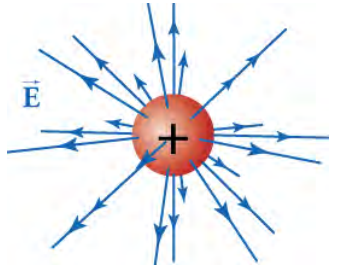
\includegraphics[width=0.8\linewidth]{phys11-electrostatics-electric-field-point-charge.png}
        \end{figure}
    
\end{frame}

\begin{frame}
    \frametitle{Electric Field Lines}
    Properties of electric field lines:
    \begin{itemize}
        \item Electric field lines \textbf{never cross} each other
        \item More field lines indicate a \textbf{stronger field}
        \item Lines \textbf{start at positive charges} and point away
        \item Lines \textbf{end at negative charges} and point toward them
        \item In free space, field lines extend to infinity
    \end{itemize}
    
    
        \begin{figure}
            \centering
            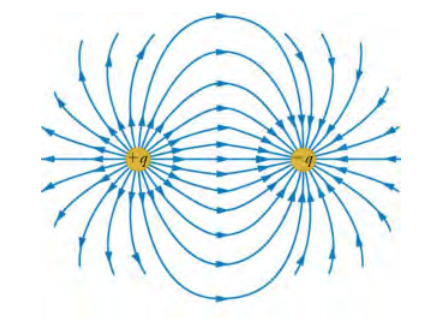
\includegraphics[width=0.5\linewidth]{phys11-electrostatics-field-lines-positive-negative-charges.png}
        \end{figure}
    
\end{frame}

\section{Electric Potential}

% Electric Potential Energy
\begin{frame}
    \frametitle{Electric Potential Energy}
    \begin{block}{Definition}
        Electric potential energy is the potential that charges have to do work by virtue of their positions relative to each other.
    \end{block}
    
    \begin{block}{Mathematical Expression}
        For a charge $q$ in the presence of a point charge $Q$:
        \begin{equation}
            U_E = \frac{kqQ}{r}
        \end{equation}
        
        Change in potential energy in constant field:
        \begin{equation}
            \Delta U_E = -qE(r_f - r_i)
        \end{equation}
    \end{block}
\end{frame}

\begin{frame}
\begin{figure}
    \centering
    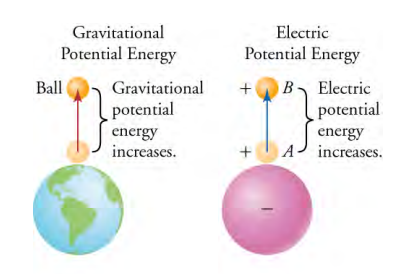
\includegraphics[width=0.75\linewidth]{phys11-energy-gravitational-vs-electric-potential.png}
\end{figure}
\end{frame}

% Electric Potential
\begin{frame}
    \frametitle{Electric Potential}
    \begin{block}{Definition}
        Electric potential is the electric potential energy per unit charge:
        \begin{equation}
            V = \frac{U_E}{q}
        \end{equation}
    \end{block}
    
    \begin{block}{Mathematical Expression}
        For a point charge $Q$:
        \begin{equation}
            V = \frac{kQ}{r}
        \end{equation}
        
        Change in potential in constant field:
        \begin{equation}
            \Delta V = -E(r_f - r_i)
        \end{equation}
    \end{block}
    \end{frame}

\begin{frame}
    
   \begin{figure}
       \centering
       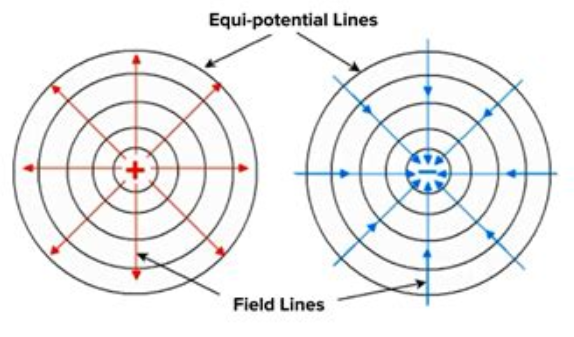
\includegraphics[width=1\linewidth]{phys11-electrostatics-equipotential-field-lines.png}
   \end{figure}
    
\end{frame}

% Movement of Charges in Potential
\begin{frame}
    \frametitle{Movement of Charges in Potential}
    \begin{block}{Key Principles}
        \begin{itemize}
            \item Potential is always measured between two points
            \item One reference point may be at infinity ($V = 0$)
            \item Charges move spontaneously to minimize potential energy:
                \begin{itemize}
                    \item \textbf{Positive charges} move from \textbf{high} to \textbf{low} potential
                    \item \textbf{Negative charges} move from \textbf{low} to \textbf{high} potential
                \end{itemize}
        \end{itemize}
    \end{block}
    \end{frame}

\begin{frame}
    
       \begin{figure}
           \centering
           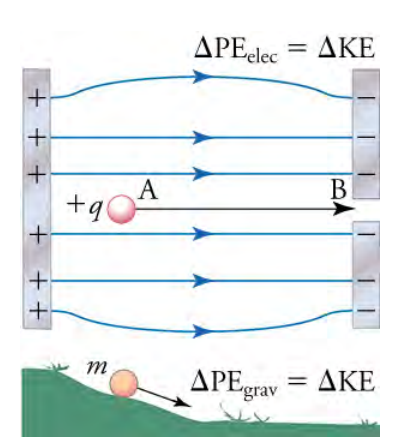
\includegraphics[width=0.6\linewidth]{jyrstgfs.png}
       \end{figure}
    
\end{frame}

\section{Capacitors and Dielectrics}

% Capacitors
\begin{frame}
    \frametitle{Capacitors}
    \begin{block}{Definition}
        A capacitor is a device that stores electric charge and energy in the electric field between its plates.
    \end{block}
    
    \begin{block}{Capacitance}
        Capacitance is the ratio of charge to potential difference:
        \begin{equation}
            C = \frac{Q}{V}
        \end{equation}
        
        Capacitance depends only on:
        \begin{itemize}
            \item Geometry of the capacitor
            \item Materials from which it is made
            \item \textbf{Does not} depend on the voltage
        \end{itemize}
    \end{block}
    \end{frame}

\begin{frame}
    
       \begin{figure}
           \centering
           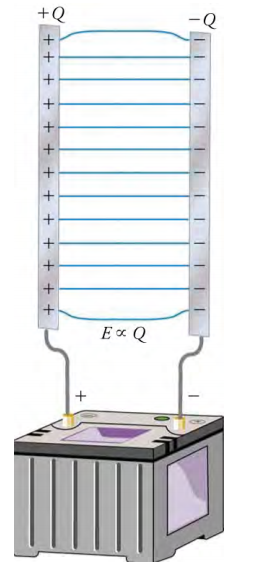
\includegraphics[width=0.25\linewidth]{phys11-electrostatics-parallel-plate-capacitor-diagram.png}
       \end{figure}
    
\end{frame}

% Parallel-Plate Capacitor
\begin{frame}
    \frametitle{Parallel-Plate Capacitor}
    \begin{block}{Capacitance Formula}
        For a parallel-plate capacitor:
        \begin{equation}
            C = \epsilon_0 \frac{A}{d}
        \end{equation}
        where:
        \begin{itemize}
            \item $\epsilon_0 = 8.85 \times 10^{-12} \, \text{F/m}$ (permittivity of free space)
            \item $A$ is the area of each plate
            \item $d$ is the separation distance between plates
        \end{itemize}
    \end{block}
    
    \begin{block}{Energy Storage}
        Energy stored in a capacitor:
        \begin{equation}
            U_E = \frac{1}{2}CV^2
        \end{equation}
    \end{block}
\end{frame}

% Dielectrics
\begin{frame}
    \frametitle{Dielectrics}
    \begin{block}{Definition}
        A dielectric material is an insulator that becomes polarized in an electric field.
    \end{block}
    
    \begin{block}{Effects of Dielectrics}
        Inserting a dielectric between capacitor plates:
        \begin{itemize}
            \item Increases the capacitance by a factor $\kappa$ (dielectric constant)
            \begin{equation}
                C = \kappa \epsilon_0 \frac{A}{d}
            \end{equation}
            \item Reduces the electric field inside the capacitor
            \item Allows for higher voltage before breakdown
        \end{itemize}
    \end{block}
    \end{frame}

\begin{frame}
    
      \begin{figure}
          \centering
          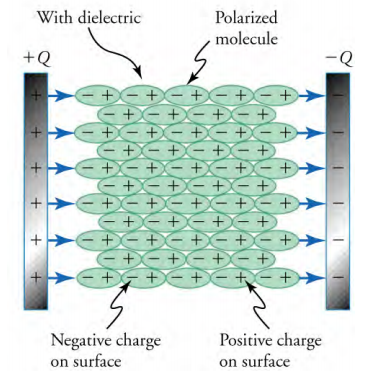
\includegraphics[width=0.7\linewidth]{phys11-electrostatics-dielectric-polarization.png}
      \end{figure}
    
\end{frame}

\section{Key Equations}

% Key Equations Summary
\begin{frame}
    \frametitle{Key Equations Summary}
    \begin{columns}
        \begin{column}{0.5\textwidth}
            \textbf{Coulomb's Law:}
            \begin{equation}
                F = \frac{kq_1q_2}{r^2}
            \end{equation}
            
            \textbf{Electric Field:}
            \begin{equation}
                E = \frac{F}{q_{\text{test}}}
            \end{equation}
            
            \textbf{Point Charge Field:}
            \begin{equation}
                E = \frac{kq}{r^2}
            \end{equation}
        \end{column}
        
        \begin{column}{0.5\textwidth}
            \textbf{Electric Potential:}
            \begin{equation}
                V = \frac{kQ}{r}
            \end{equation}
            
            \textbf{Capacitance:}
            \begin{equation}
                C = \frac{Q}{V}
            \end{equation}
            
            \textbf{Parallel-Plate Capacitor:}
            \begin{equation}
                C = \epsilon_0 \frac{A}{d}
            \end{equation}
            
            \textbf{Energy Storage:}
            \begin{equation}
                U_E = \frac{1}{2}CV^2
            \end{equation}
        \end{column}
    \end{columns}
\end{frame}

\section{Examples}

% "I do" Example
\begin{frame}
    \frametitle{"I do" Example: Coulomb's Law}
    \begin{block}{Problem}
        Two point charges $q_1 = +2.0 \, \mu\text{C}$ and $q_2 = -3.0 \, \mu\text{C}$ are separated by a distance of $0.15 \, \text{m}$. Find the magnitude and direction of the electric force between them.
    \end{block}
    \pause
    \begin{block}{Solution}
        Using Coulomb's law: $F = \frac{kq_1q_2}{r^2}$
        
        $F = \frac{(9 \times 10^9 \, \text{N} \cdot \text{m}^2/\text{C}^2)(2.0 \times 10^{-6} \, \text{C})(-3.0 \times 10^{-6} \, \text{C})}{(0.15 \, \text{m})^2}$
        
        $F = \frac{(9 \times 10^9)(-6.0 \times 10^{-12})}{0.0225}$
        
        $F = -2.4 \times 10^{-3} \, \text{N}$
        
        The negative sign indicates an attractive force. The force on $q_1$ is directed toward $q_2$, and the force on $q_2$ is directed toward $q_1$.
    \end{block}
\end{frame}

% "We do" Example
\begin{frame}
    \frametitle{"We do" Example: Electric Field}
    \begin{block}{Problem}
        Three point charges are arranged on the x-axis: $q_1 = +2.0 \, \mu\text{C}$ at $x = 0$, $q_2 = -3.0 \, \mu\text{C}$ at $x = 0.15 \, \text{m}$, and $q_3 = +1.0 \, \mu\text{C}$ at $x = 0.30 \, \text{m}$. Find the electric field at point P located at $x = 0.45 \, \text{m}$.
    \end{block}
        \pause

    \begin{block}{Solution Approach}
        1. Calculate the electric field due to each charge at point P
        \begin{align}
            E_1 &= \frac{kq_1}{r_1^2} = \frac{k(+2.0 \times 10^{-6})}{(0.45)^2} \text{ (pointing right)} \\
            E_2 &= \frac{kq_2}{r_2^2} = \frac{k(-3.0 \times 10^{-6})}{(0.30)^2} \text{ (pointing left)} \\
            E_3 &= \frac{kq_3}{r_3^2} = \frac{k(+1.0 \times 10^{-6})}{(0.15)^2} \text{ (pointing right)}
        \end{align}
        
        2. Find the total field by superposition: $\vec{E}_{\text{total}} = \vec{E}_1 + \vec{E}_2 + \vec{E}_3$
    \end{block}
\end{frame}

% "You do" Example
\begin{frame}
    \frametitle{"You do" Example: Capacitor}
    \begin{block}{Problem}
        A parallel-plate capacitor has plates with an area of $0.0025 \, \text{m}^2$ separated by a distance of $0.5 \, \text{mm}$. 
        
        (a) Calculate the capacitance of this capacitor.
        
        (b) If the capacitor is connected to a $12 \, \text{V}$ battery, determine the charge stored on each plate.
        
        (c) Calculate the energy stored in the capacitor.
        
        (d) If a dielectric with $\kappa = 3.0$ is inserted between the plates, find the new capacitance.
    \end{block}
    
    \begin{block}{Hints}
        \begin{itemize}
            \item Use $C = \epsilon_0 \frac{A}{d}$ for part (a)
            \item Apply $Q = CV$ for part (b)
            \item Use $U_E = \frac{1}{2}CV^2$ for part (c)
            \item Remember that with a dielectric, $C = \kappa\epsilon_0 \frac{A}{d}$
        \end{itemize}
    \end{block}
\end{frame}

\section{Summary}

% Summary
\begin{frame}
    \frametitle{Summary: Key Takeaways}
    \begin{block}{Electrical Charges \& Coulomb's Law}
        \begin{itemize}
            \item Electric charge is conserved; like charges repel, unlike attract
            \item Coulomb's law: $F = \frac{kq_1q_2}{r^2}$
        \end{itemize}
    \end{block}
    
    \begin{block}{Electric Field \& Potential}
        \begin{itemize}
            \item Electric field: force per unit charge; $E = \frac{F}{q_{\text{test}}}$
            \item Electric potential: potential energy per unit charge; $V = \frac{U_E}{q}$
        \end{itemize}
    \end{block}
    
    \begin{block}{Capacitors \& Dielectrics}
        \begin{itemize}
            \item Capacitance $C = \frac{Q}{V}$; energy storage $U_E = \frac{1}{2}CV^2$
            \item Parallel-plate capacitor: $C = \epsilon_0 \frac{A}{d}$
            \item Dielectrics increase capacitance by a factor $\kappa$
        \end{itemize}
    \end{block}
\end{frame}

% End Slide
\begin{frame}
    \frametitle{Thank You!}
    \begin{center}
        \Large Questions?
        
        \vspace{1cm}
        
        \normalsize Practice problems: Textbook Chapter 18 
    \end{center}
\end{frame}

\end{document}